\begin{table*}[t]\centering
\caption{Accuracy at validation-best checkpoints, with final-epoch test accuracy for comparison. Mean $\pm$ sample SD across three paired seeds; all accuracies and gaps are in percentage points. Muon+ denotes the hybrid.}
\label{tab:accuracy}
\begin{tabular}{lrrrrrr}\toprule
Method & Selected LR & Train & Validation & Test & Train--test gap & Final test\\\midrule
SGD-M & 0.03 & \pmv{91.08}{0.77} & \pmv{88.82}{0.15} & \pmv{87.57}{0.32} & \pmv{3.51}{0.52} & \pmv{87.52}{0.51}\\
Adam & 0.001 & \pmv{92.01}{0.62} & \pmv{88.97}{0.47} & \pmv{88.32}{0.40} & \pmv{3.70}{0.25} & \pmv{88.05}{0.41}\\
AdamW & 0.001 & \pmv{92.68}{0.52} & \pmv{89.33}{0.15} & \pmv{88.59}{0.18} & \pmv{4.09}{0.35} & \pmv{88.55}{0.30}\\
Muon+AdamW & 0.005 & \pmv{94.03}{1.21} & \pmv{89.73}{0.21} & \pmv{89.04}{0.29} & \pmv{4.99}{0.92} & \pmv{88.97}{0.14}\\
\bottomrule\end{tabular}\end{table*}
\begin{figure*}[t]\centering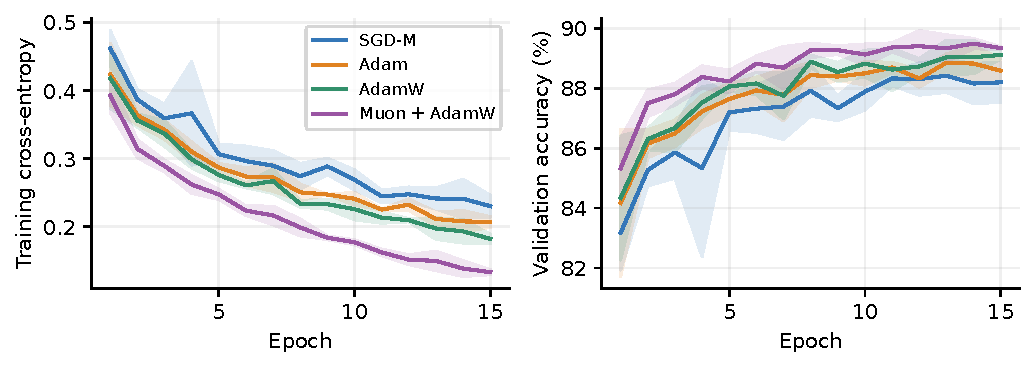
\includegraphics[width=.96\textwidth]{figures/convergence.pdf}
\caption{Training-set loss at epoch-end checkpoints and validation accuracy at equal epochs/updates. Lines are means; bands show one sample standard deviation over three seeds.}\label{fig:convergence}\end{figure*}
